\section{Lecture 25}
\subsection{Lecture Notes - The Poisson Brackeet and Liouville's Theorem}
\subsubsection{Review}
On Monday, we talked about canonical transformations. In Lagrangian picture, we found that Lagrange's equation of motion were invaraint under coordinate transformations. In Hamilton's picture, $p$ and $q$ play the same role. In the phase space spanned by $p$ and $q$, there are a wider class of possible transformations that can be made. Not all of these transformations leave Hamilton's equations invariant. The subclass that do is called canaonical. Adding he total time derivative of a function $F$ is what could accomplish this. 

\subsubsection{Poisson Bracket}
Consider the phase space function $F(q, p, t)$ (any function of the variables of phase space, could depend on time, could be energy, angular momentum etc.). Let us write the total time derivative of this. As usual, we expand this total derivative to get:
\[\dod{F}{t} = \sum_j \dpd{F}{q_j}\dot{q}_j + \sum_j\dpd{F}{p_j}\dot{p}_j + \dpd{F}{t}\]
Using Hamilton's equations to replace $\dot{q}_j$ and $\dot{p}_j$, we get that:
\[\dod{F}{t} = \sum_j\dpd{F}{q_j}\dpd{\HH}{p_j} - \sum_j\dpd{F}{p_j}\dpd{\HH}{q_j} + \dpd{F}{t}\]
We may write this as:
\[[F, H] + \dpd{F}{t}\]
This is the \textbf{Poisson Bracket}. It's a shorthand for $\sum_j\pd{F}{q_j}\pd{\HH}{p_j} - \sum_j\pd{F}{p_j}\pd{\HH}{q_j}$. As a note of notation, it can also be written with curly brackets \{ \}. If $F$ is conserved, an equivalent statement is that $\dod{F}{t} = 0$, and equivalent to this is that $[F, H] = 0$. 

\subsubsection{Properties of the Poisson Bracket}
\begin{enumerate}
    \item Anti-symmetry $[F, G] = -[G, H]$, from which we obtain $[F, F] = 0$.
    \item Bilinearity $[aF + bG, H] = a[F, H] + b[G, H]$ and $[H, aF + bG] = a[H, F] + b[H, G]$
    \item Leibniz' Rule $[FG, H] = [F, H]G + F[G, H]$
    \item Jacobi Identity $[F, [G, H]] + [G, [H, F]] + [H, [F, G]] = 0$
\end{enumerate}

\subsubsection{Poisson Bracket and Canonical Transformations}
We test if the following transformation is canonical:
\[q_i \mapsto Q_i(p, q), \quad p_i \mapsto P_i(p, q), \quad \dpd{F}{t} = 0, \quad K = \HH\]
We claim that this is the case if the following identities hold for the fundamental Poisson brackets:
\[[Q_i, Q_l] = 0, \quad [P_i, P_l] = 0, \quad [Q_i, P_l] = \delta_{il}\]
are obeyed. As a remark, these identities are \textit{quite} similar to the canonical commutation relations that we see in quantum mechanics. This shows that the structure in phase space is ready to be quantized. But, we return to this on Friday. For now, we return to the proof. Taking the total time derivative of $F$, we have:
\[\dod{F}{t} = \ldots = \sum_l \dpd{K}{Q_l}[F, Q_l] + \sum_l \dpd{K}{P_l}[F, P_l]\]
These identities were just obtained by the chain rule and reordering. We now consider some cases. In the first case, consider $F = Q_i$. In this case,
\[\dot{Q}_i = \sum_l\dpd{K}{Q_l}[Q_i, Q_l] + \sum_l\dpd{K}{P_l}[Q_i, P_l]\]
In order for Hamilton's equation to be satisfied, we require that this expression is equal to $\dpd{K}{P_i}$. From this, we require that $[Q_i, Q_l] = 0$, and $[Q_i, P_l] = \delta_{il}$. In the second case, consider $F =P_i$. Then,
\[\dot{P}_i = \sum_l\dpd{K}{Q_l}[P_i, Q_l] + \sum_l\dpd{K}{P_l}[P_i, P_l]\]
Again, in order for Hamilton's equations to be satisfied, we require that this is equal to $-\dpd{K}{Q_i}$. From this we obtain that $[P_i, Q_l] = -\delta_{il}$, and $[P_i, P_l] = 0$. This completes the proof of the claim. \\
We also see that
\[\dot{q_i}=[q_i, \HH], \quad \dot{p_i}=[p_i, \HH]\]
Since
\[\dot{q_i}=[q_i, \HH]=\sum_k \underbrace{\dpd{q_i}{q_k}}_{=\delta_{ik}} \dpd{\HH}{p_k}-\sum_k \underbrace{\dpd{q_i}{p_k}}_{=0} \dpd{\HH}{q_k}=\dpd{\HH}{p_i}\]
\[\dot{p_i}=[p_i, \HH]=\sum_k \underbrace{\dpd{p_i}{q_k}}_{=0} \dpd{\HH}{p_k}-\sum_k \underbrace{\dpd{p_i}{p_k}}_{=\delta_{ik}} \dpd{\HH}{q_k}=-\dpd{\HH}{q_i}\]

\subsubsection{Hamiltonian Flow}
Recall our discussion of the phase space vector:
\[\v{z} = \m{\v{q} \\ \v{p}}\]
Which in general has $2n$ elements for $n$ degrees of freedom (recall the 2d phase space vector for the 1-dimensional harmonic oscillator). Taking the time derivative of this, we get the phase space velocity vector:
\[\dot{\v{z}} = \m{\dot{\v{q}} \\ \dot{\v{p}}} = \m{\dpd{\HH}{\v{p}} \\ -\dpd{\HH}{\v{q}}} = \v{v}(\v{z})\]
The idea is that the phase space trajectories depend on the total energy of the system. For example with the double well potential:
\begin{center}
    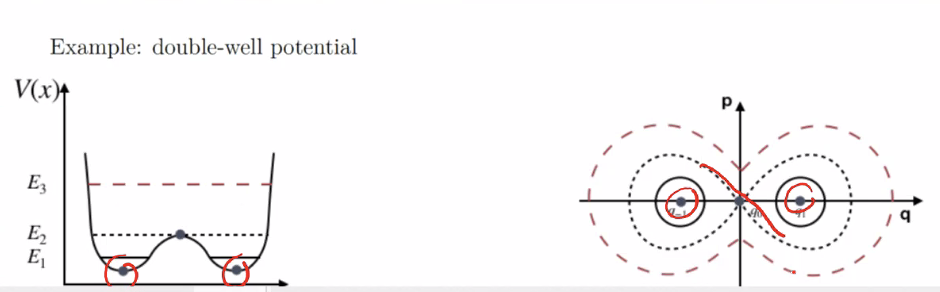
\includegraphics[scale=0.8]{Lecture-25/l25-img1.png}
\end{center}
Now, let us consider a bunch of systems that are some time close together (in phase space):
\begin{center}
    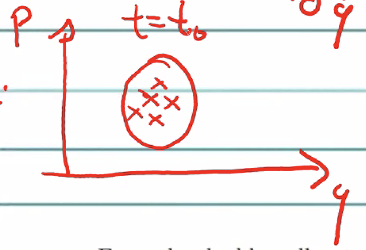
\includegraphics[scale=0.8]{Lecture-25/l25-img2.png}
\end{center}
What happens to this cloud of points as it goes through a time evolution? These trajectories are unique and deterministic, so at some later point in time, this cloud may have moved in phase space. It also does not have to have the same shape. But, the points inside the cloud have to stay inside the cloud, as trajectories cannot cross in Hamiltonian dynamics. Points inside stay on the inside.
\begin{center}
    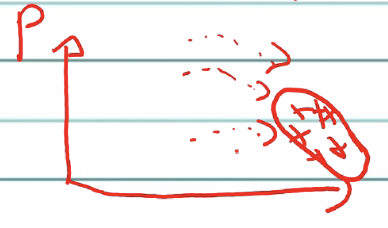
\includegraphics[scale=0.8]{Lecture-25/l25-img3.png}
\end{center}
In general, there is a hyper-volume (the cloud) in phase space, which moves through the space with time; this is the picture we want to have when thinking about Hamiltonian flow. 

\subsubsection{Liouville's Theorem}
We hence consider a map:
\[\v{z}_0 \mapsto \v{z}(t)\]
which is the definition of the Hamiltonian/phase space flow. The statement of Liouville's theorem is that the area initially occupied by the cloud in phase space is the same as the area occupied at some point later (for higher dimensions, replace area with hyper-volume). 
\begin{center}
    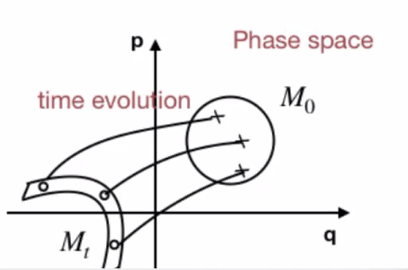
\includegraphics[scale=0.8]{Lecture-25/l25-img4.png}
\end{center}
We will make this statement more precise as we go on. In order to see this, we again look at this Hamiltonian flow. Hamilton's equations are a description/map of these positions in phase space to a later time. Let us examine the properties of this map for a small time interval:
\[q_i \mapsto Q_i = q_i + \dot{q}_idt\]
\[p_i \mapsto P_i = p_i + \dot{p}_idt\]
This is of course just a first-order Taylor expansion/linear approximation. Of course we can rewrite these expressions using Hamilton's equations:
\[q_i \mapsto q_i + \dpd{\HH}{p_i}dt\]
\[p_i \mapsto p_i - \dpd{\HH}{q_i}dt\]
The statement of Liouville's theorem can then be made to say:
\[V_{pq} = d\v{q}d\v{p} = V_{PQ} = d\v{P}d\v{Q}\]
What happens if we apply this transformation and compare? This is just a statement about a change of variables. Let us recall what we did for integration. When switching integration variables $x = x(u, v)$, $y = y(u, v)$, which of the following is correct?
\begin{s}
We recall how we did coordinate transformations using the Jacobian:
\[\iint f(x, y)dxdy = \iint f(x(u, v), y(u, v)) \abs{\dpd{(x,y)}{(u, v)}}dudv\]
Note that here $\abs{\dpd{(x,y)}{(u, v)}}$ is the determinant of the 2x2 matrix containing the partial derivatives (the determinant of the Jacobian), e.g.:
\[\dpd{(x,y)}{(u, v)} = \m{\dpd{x}{u} & \dpd{x}{v} \\ \dpd{y}{u} & \dpd{y}{v}}\]
Hence, returning to our discussion of the conserved volumes; we can write $d\v{P}d\v{Q}$ as:
\[V_{pq} = d\v{q}d\v{p} = V_{PQ} = d\v{P}d\v{Q} = \abs{\dpd{\v{z}_t}{\v{z}_0}}d\v{p}d\v{q}\]
We can write this Jacobian as:
\[\dpd{\v{z}_t}{\v{z}_0} = \m{\dpd{Q}{q} & \dpd{Q}{p} \\ \dpd{P}{q} & \dpd{P}{p}} = \m{1 + \pdv{\HH}{p}{q}dt & \dpd[2]{\HH}{p}dt \\ -\dpd[2]{\HH}{p}dt & 1 - \pdv{\HH}{p}{q}dt }\]
We have done this many times in the past, e.g. when transforming from cartesian to spherical coordinates. The factor $r^2\sin\theta$ in this coordinate transformation from cartesian to spherical is the determinant of the Jacobian in that case. Here, we are just transforming from a system at time $t = 0$ to time $t = t$. Hence taking the determinant, we have:
\[\abs{\dpd{\v{z}_t}{\v{z}_0}} = 1 - \left(\pdv{\HH}{p}{q}\right)^2dt^2 + \dpd[2]{\HH}{p}\dpd[2]{\HH}{q}dt^2 + \cdots \]
We note that there are no linear terms in $dt$. Hence, the time derivative of this object is zero. Hence, the phase space volume does not change. Equivalently, $\od{V}{t} = 0$. The fluid of phase space moves like an incompressable fluid, keeping its volume. 
\end{s} 